\documentclass[11pt]{beamer}
\usepackage[utf8]{inputenc}
\usepackage[spanish]{babel}
\usepackage{amsmath}
\usepackage{amsfonts}
\usepackage{amssymb}
\usepackage{graphicx}
\usepackage{lipsum}
\usepackage{ragged2e}
\usepackage{hyperref}
\usepackage{float}
\usepackage{url}
\usetheme{Madrid}
\newcommand{\celda}[1]{
	\begin{minipage}{2.5cm}
		\vspace{5mm}
		#1
		\vspace{5mm}
	\end{minipage}
}

\author[Grupo 1]{Landolfi Cano, Silvia \& López Gallo, Ismael \& López García, Álvaro \& Rodríguez de Frutos, Pablo \\ \textbf{Grupo 1}}
\title[Trabajo Optimización]{Optimización mediante el problema de una pompa de jabón apoyada entre dos circunferencias paralelas y coaxiales}
\date{\today} 
\logo{
\includegraphics[height=0.5cm]{Figuras/etsiae_logo.png}}
\institute[CO]{
        Asignatura de Control y Optimización \\
        3$^{er}$ Curso de Grado en Ingeniería Aeroespacial, especialidad CTA \\
        Escuela Técnica Superior de Ingeniería Aeronáutica y del Espacio (UPM)
	% \inst{1}
	% 	Universidad Nacional Mayor de San Marcos. Facultad de Ciencias Matemáticas. \\Escuela Profesional de Computación Científica\\
	% 	\vspace{2mm}
	% \inst{2}
	% 	Universidad Nacional Mayor de San Marcos. Facultad de Ciencias Matemáticas. \\Escuela Profesional de Estadística
}

\AtBeginSection[]
{
	\begin{frame}<beamer>{Contenido}
		\tableofcontents[currentsection,currentsubsection]
	\end{frame}
}


\begin{document}
	
	\begin{frame}
		\maketitle
	\end{frame}

	\begin{frame}{Contenido}
		\tableofcontents
	\end{frame}

	\section{Resumen}
		\begin{frame}{Resumen}
			\justifying
                En este trabajo se propone la optimización de la superficie de un fluido mediante el problema de una pompa de jabón que se apoya en dos circunferencias paralelas y coaxiales, que actúan como soporte.
                \begin{figure}
                    \centering
                    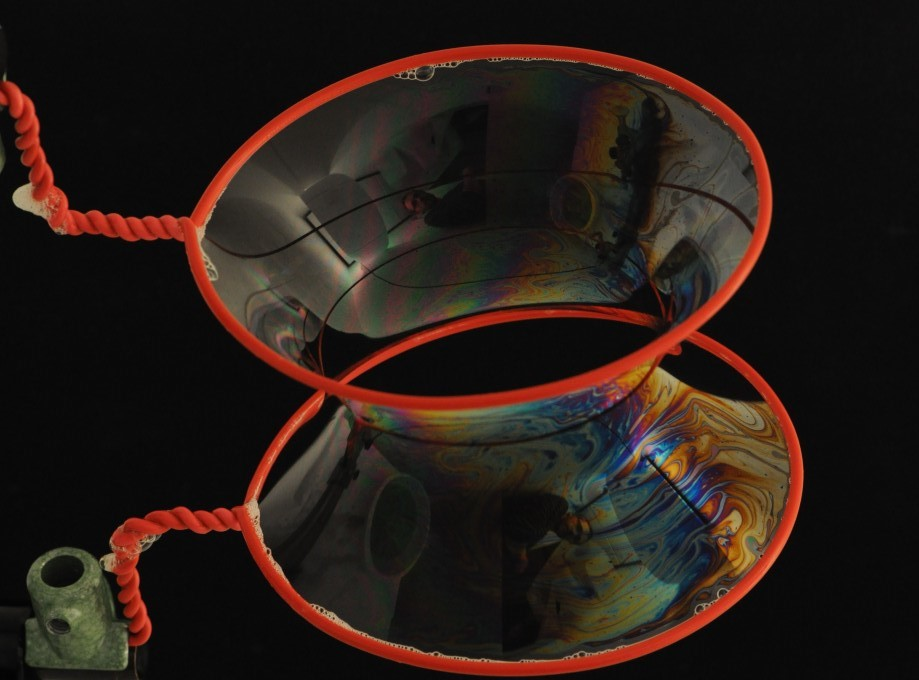
\includegraphics[width= 0.6 \textwidth, height=\textheight, keepaspectratio]{Figuras/soap_film.jpg}
                \end{figure}
		\end{frame}
	
	\section{Introducción}
		\begin{frame}{Introducción}
			\justifying
			En 2D:
                \begin{equation*}
                    A = \int_0^1 F \sqrt{1 + \left( \frac{dF}{dz} \right)^2} dz , \qquad F(z = 0) = F(z = 1) = F_0
                \end{equation*}
                Con solución analítica, la \textbf{catenaria}:
                \begin{figure}
                    \centering
                    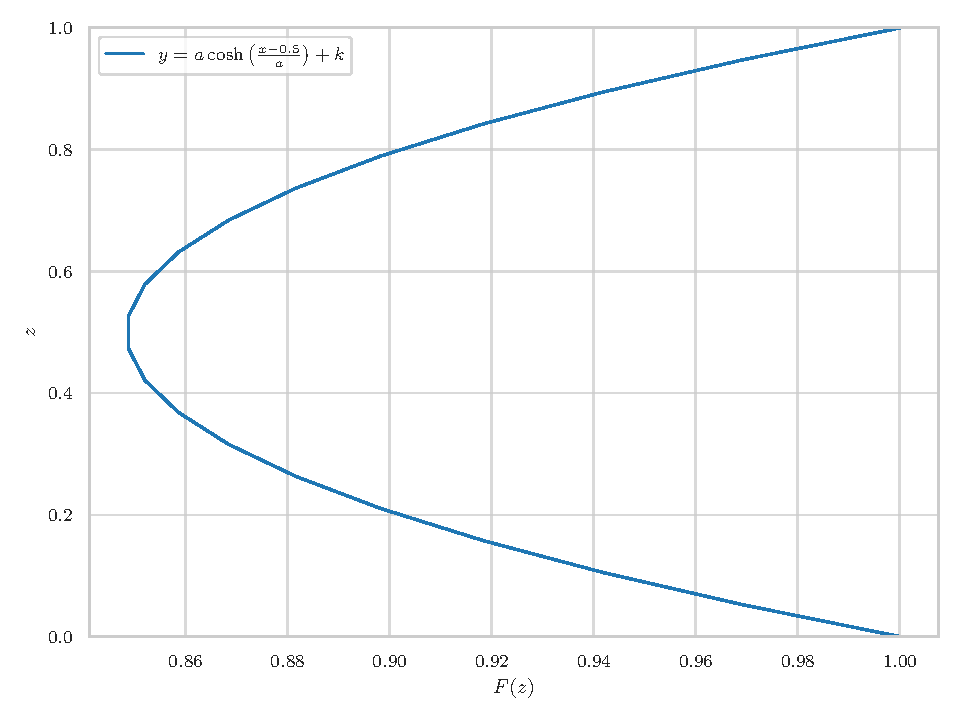
\includegraphics[width= 0.6 \textwidth, height=\textheight, keepaspectratio]{Figuras/catenaria.pdf}
                \end{figure}
		\end{frame}
  		
		\begin{frame}{Introducción}
            \framesubtitle{Problema considerado}
			\justifying
			\begin{figure}
                    \centering
                    \includegraphics[width= \textwidth, height=\textheight, keepaspectratio]{Figuras/comparacion_heuristicos_gradiente.pdf}
                \end{figure}
		\end{frame}

            \begin{frame}{Introducción}
            \framesubtitle{Métodos de optimización}
			\justifying
			Casos a considerar:
                \begin{enumerate}
                    \item Optimización sin restricciones
                    \item Optimización con restricciones de volumen:
                    \item Optimización con soportes de diferente tamaño
                \end{enumerate}

                Influencia de parámetros:
                \begin{itemize}
                    \item $F_0$
                    \item $n$
                    \item Distribución de puntos
                    \item Esquema de cálculo de derivadas
                    \item Valor de arranque
                \end{itemize}
		\end{frame}
	
	\section{Problema sin restricciones}
		\begin{frame}{Problema sin restricciones}
			\justifying
			\begin{minipage}[b]{0.48\textwidth}
                    \centering
                    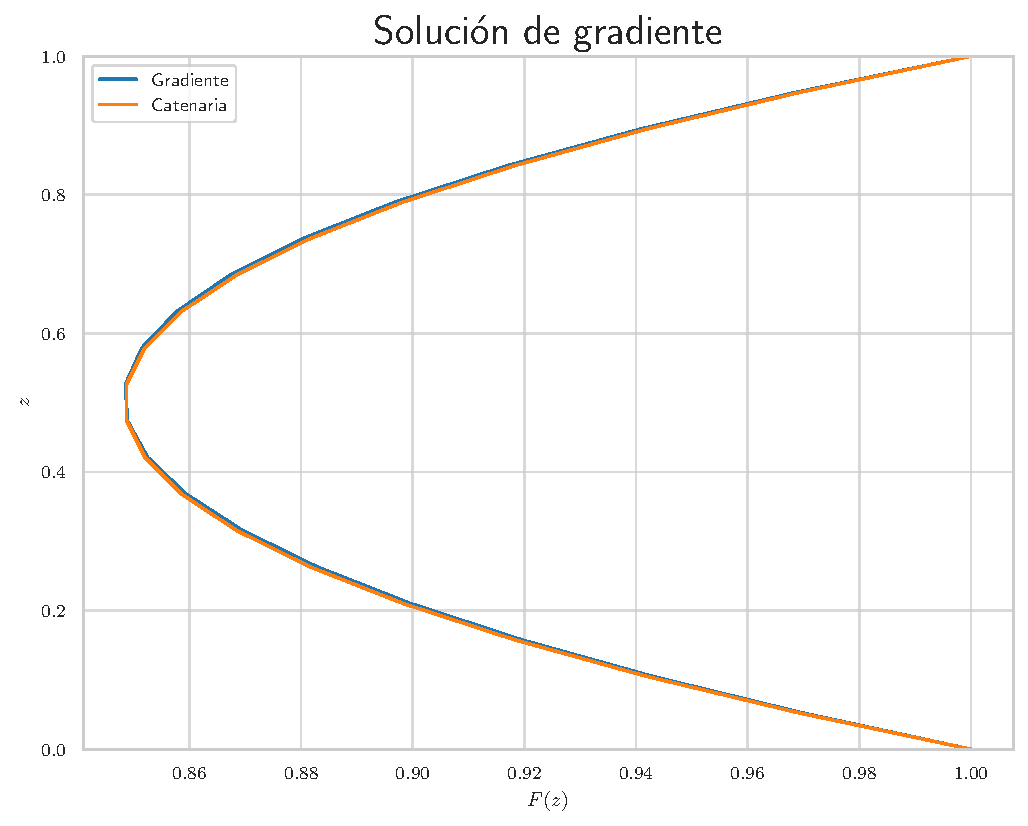
\includegraphics[height=0.5 \textheight]{Figuras/comp_grad_cat.pdf}
                \end{minipage}
                \hfill
                \begin{minipage}[b]{0.48\textwidth}
                    \centering
                    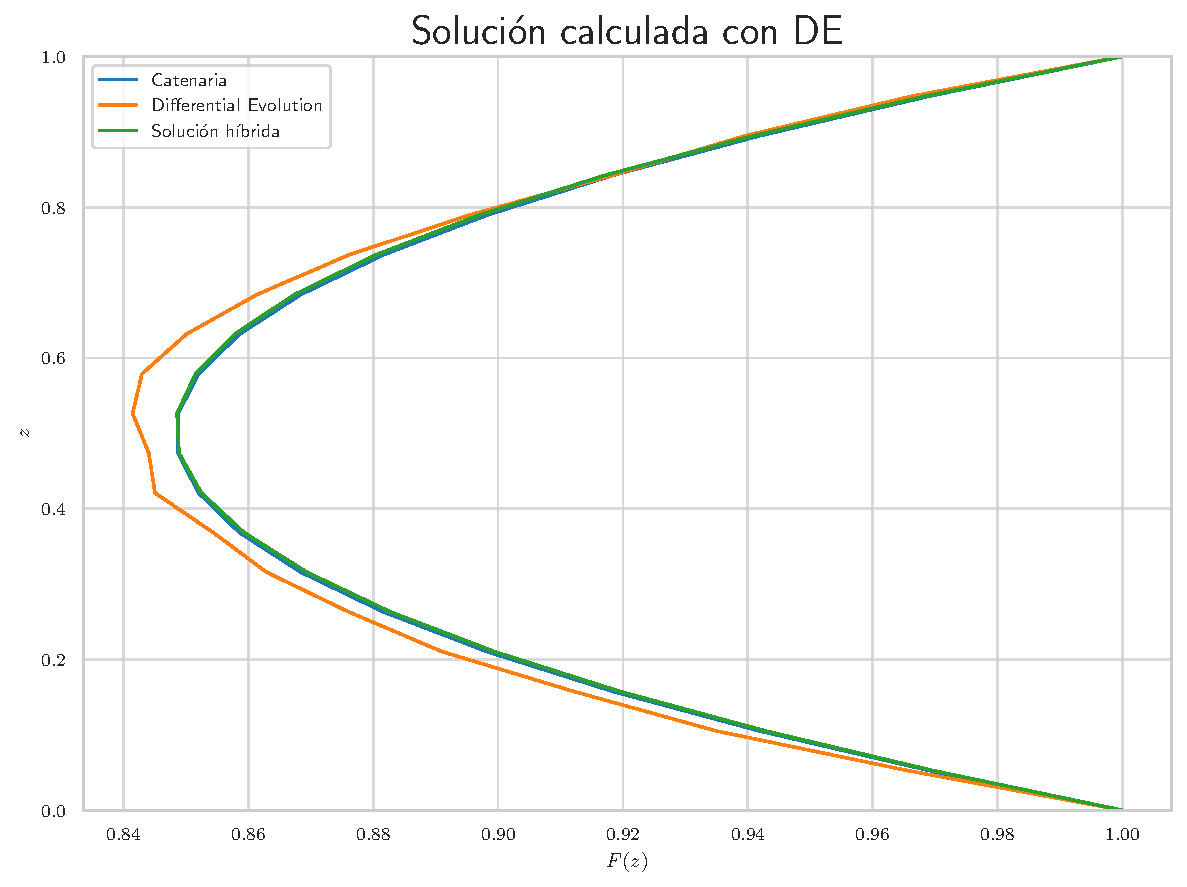
\includegraphics[height=0.5 \textheight]{Figuras/comp_de_cat.pdf}
                \end{minipage}
		\end{frame}
	
		\begin{frame}{Influencia del radio de los soportes}
			\justifying
			\begin{minipage}[b]{0.48\textwidth}
                    \centering
                    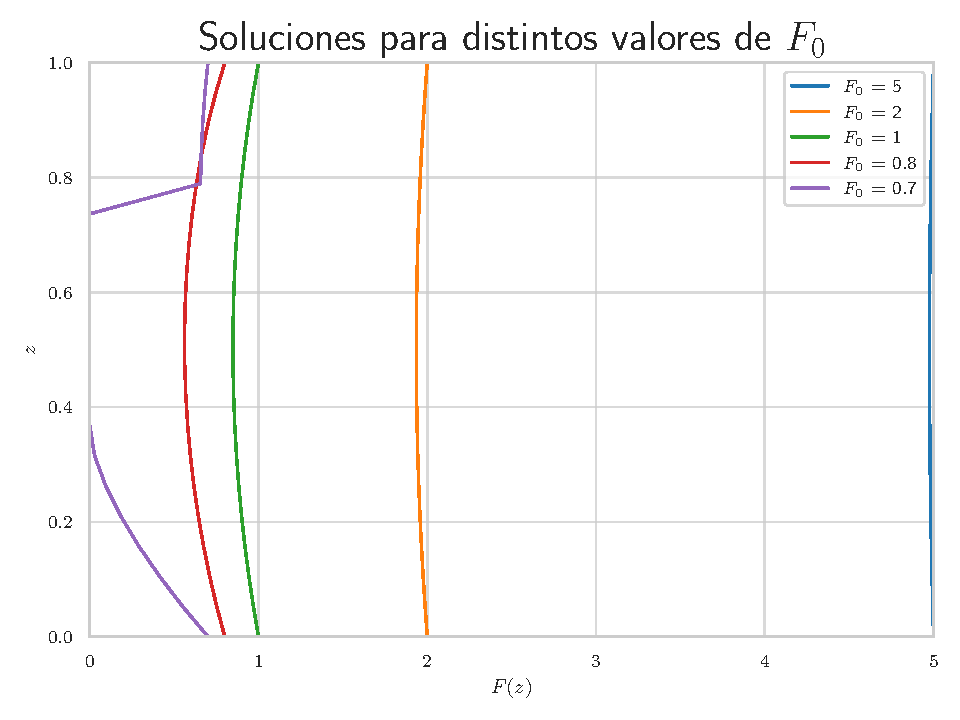
\includegraphics[height=0.5 \textheight]{Figuras/sol_radios.pdf}
                \end{minipage}
                \hfill
                \begin{minipage}[b]{0.48\textwidth}
                    \centering
                    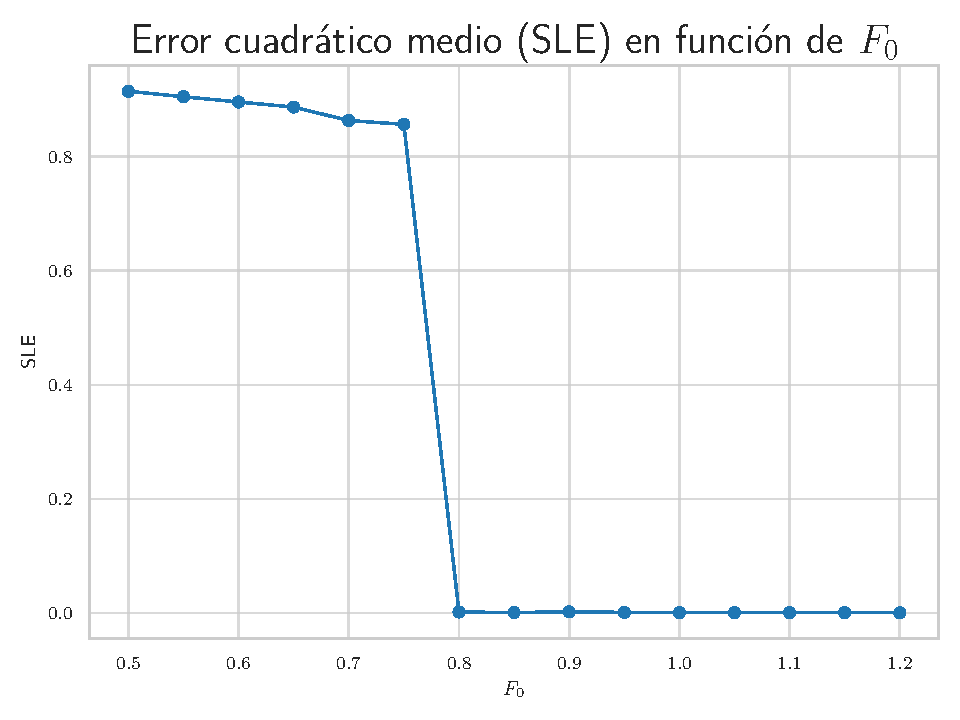
\includegraphics[height=0.5 \textheight]{Figuras/error_radios.pdf}
                \end{minipage}
		\end{frame}

            \begin{frame}{Influencia del número de puntos}
			\justifying
			\begin{minipage}[b]{0.48\textwidth}
                    \centering
                    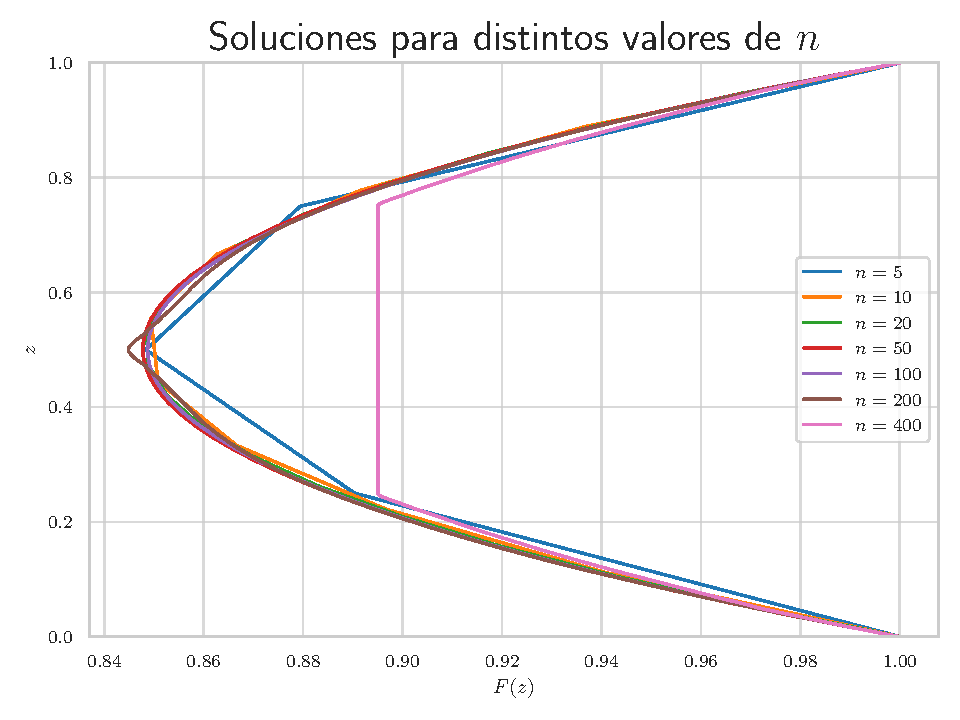
\includegraphics[height=0.5 \textheight]{Figuras/sol_n.pdf}
                \end{minipage}
                \hfill
                \begin{minipage}[b]{0.48\textwidth}
                    \centering
                    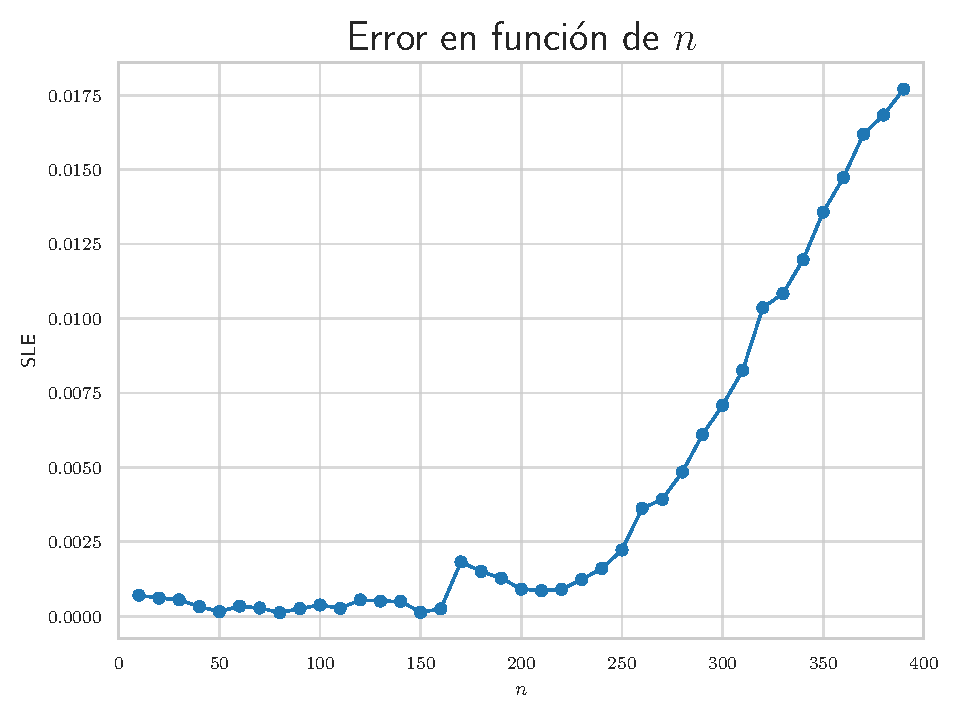
\includegraphics[height=0.5 \textheight]{Figuras/error_n.pdf}
                \end{minipage}
		\end{frame}

            \begin{frame}{Influencia de la distribución de puntos}
            % \framesubtitle{$n = 10$}
			\justifying
			\begin{minipage}[b]{0.48\textwidth}
                    \centering
                    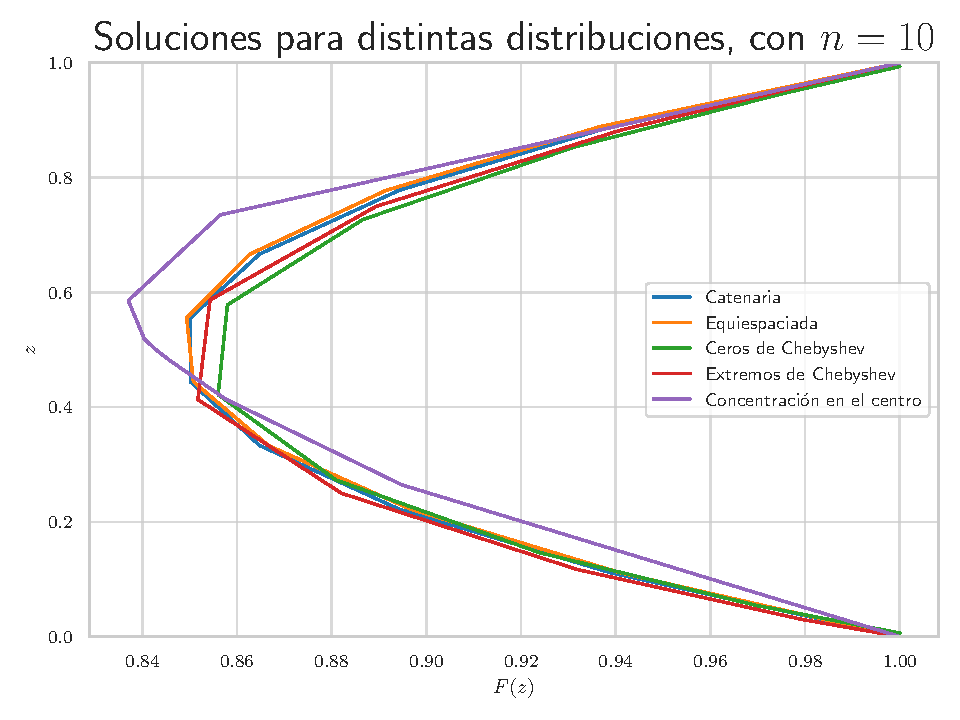
\includegraphics[height=0.5 \textheight]{Figuras/sol_distrib_n10.pdf}
                \end{minipage}
                \hfill
                \begin{minipage}[b]{0.48\textwidth}
                    \centering
                    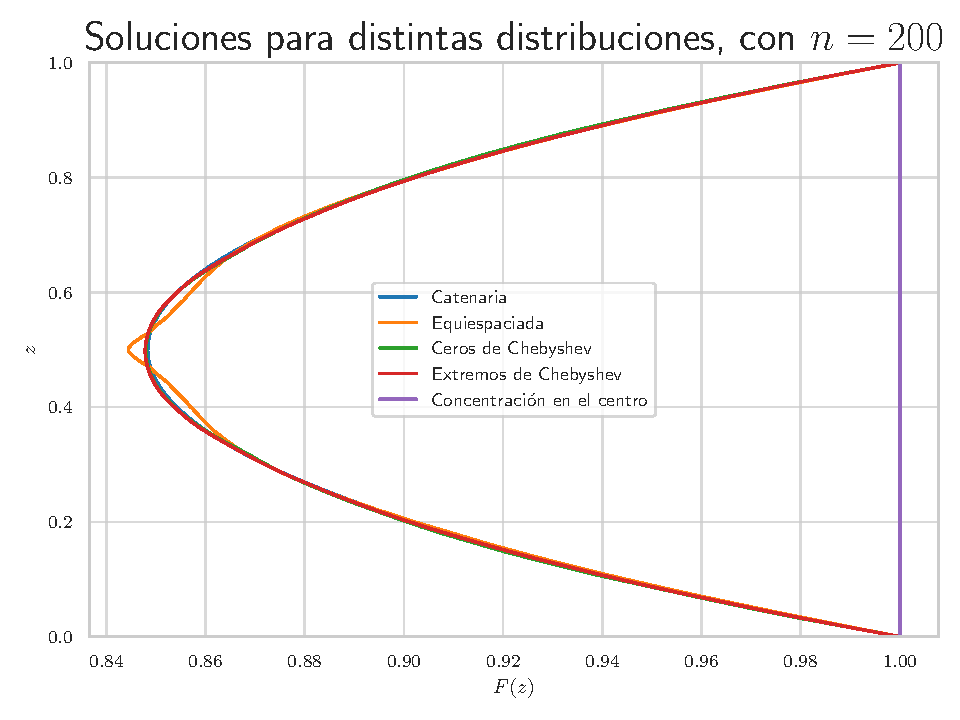
\includegraphics[height=0.5 \textheight]{Figuras/sol_distrib_n200.pdf}
                \end{minipage}
		\end{frame}

            \begin{frame}{Influencia del esquema de cálculo de derivadas}
                \begin{minipage}[b]{0.43\textwidth}
                    \centering
                    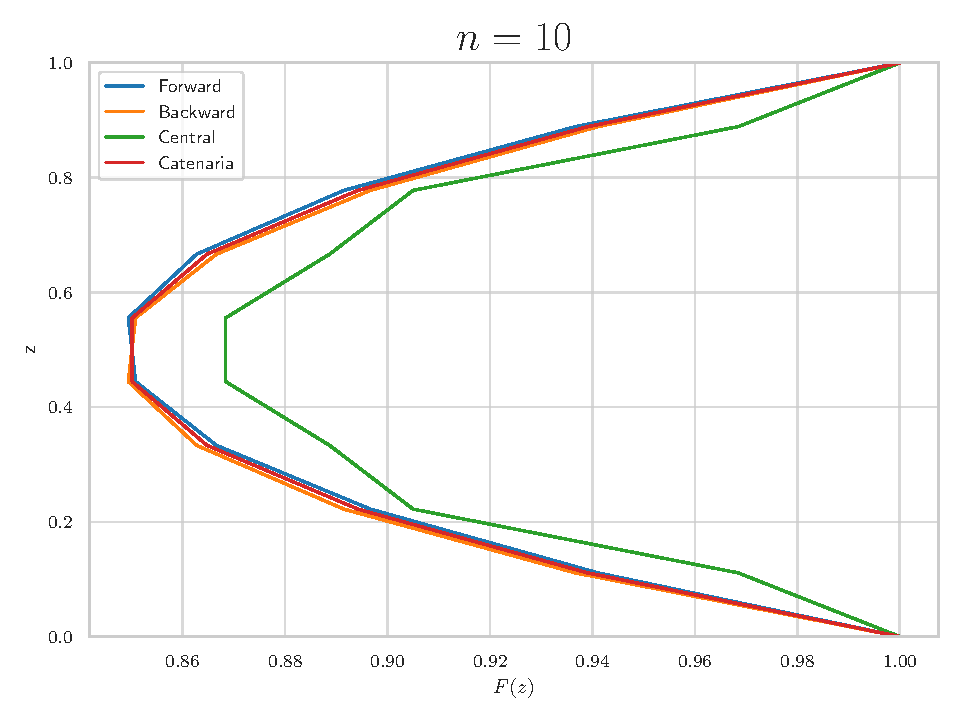
\includegraphics[width=\textwidth]{Figuras/sol_deriv_n10.pdf}
                \end{minipage}
                \hfill
                \begin{minipage}[b]{0.43\textwidth}
                    \centering
                    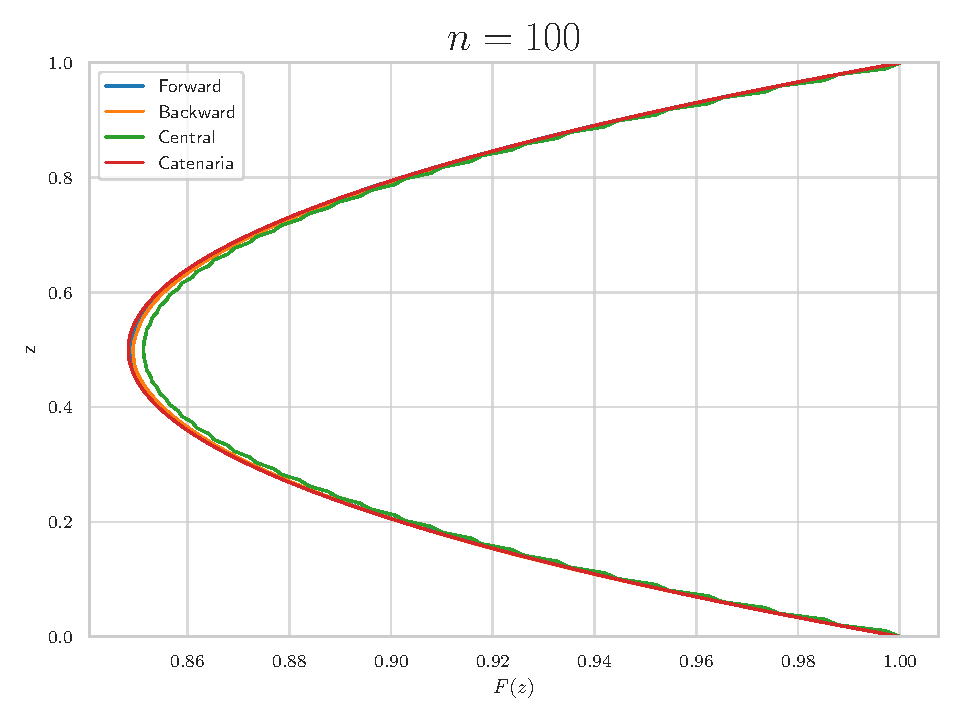
\includegraphics[width=\textwidth]{Figuras/sol_deriv_n100.pdf}
                \end{minipage}
            
                \vspace{0.1cm} % Espacio vertical entre las filas
            
                \begin{minipage}[b]{0.43\textwidth}
                    \centering
                    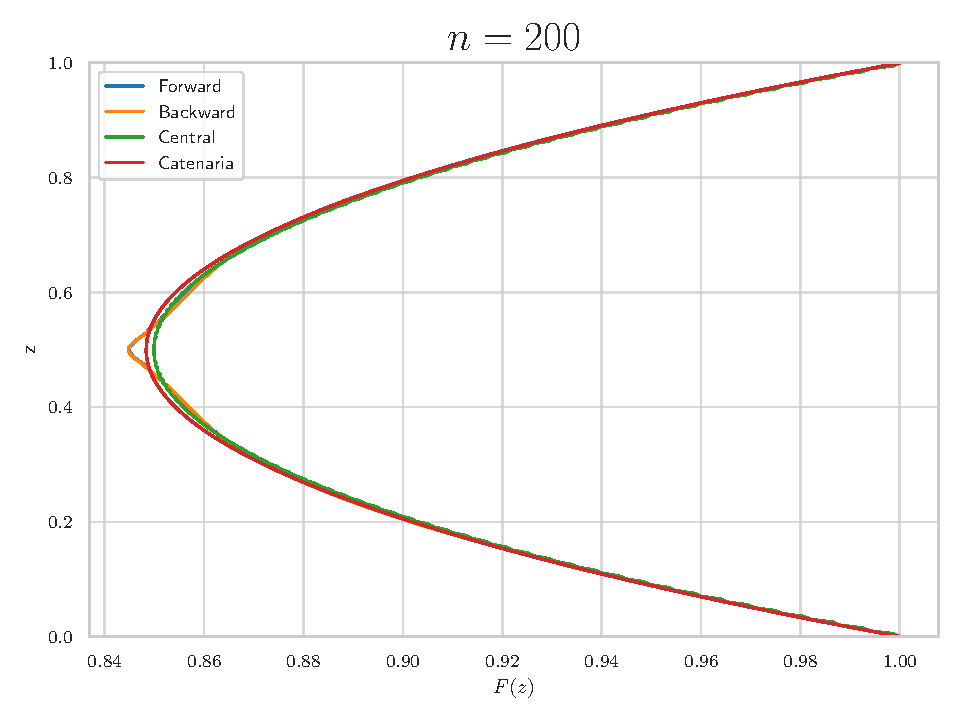
\includegraphics[width=\textwidth]{Figuras/sol_deriv_n200.pdf}
                \end{minipage}
                \hfill
                \begin{minipage}[b]{0.43\textwidth}
                    \centering
                    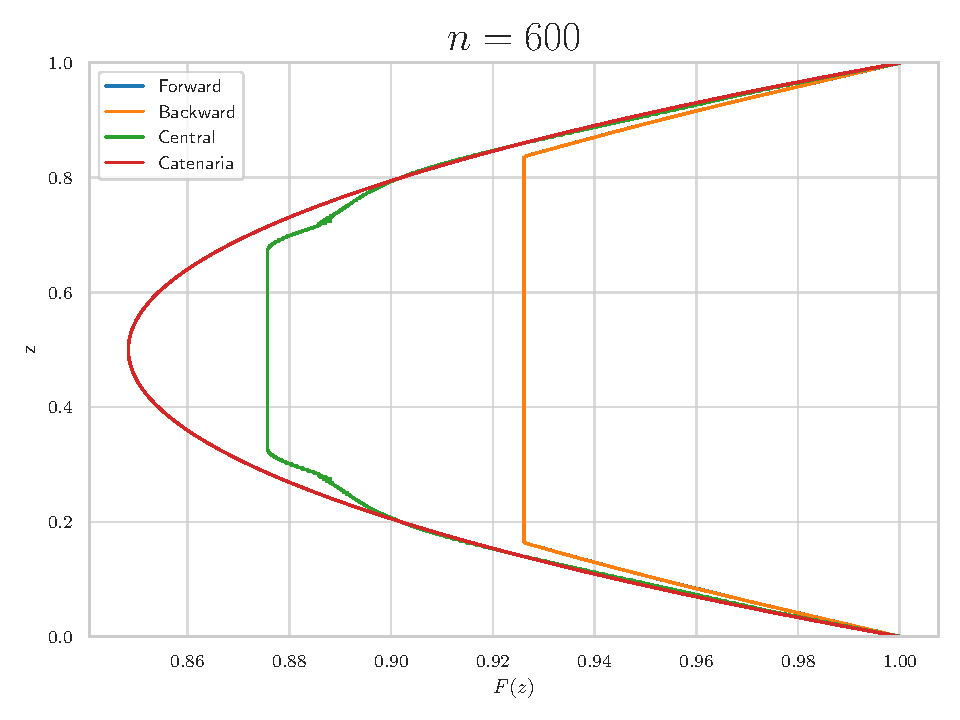
\includegraphics[width=\textwidth]{Figuras/sol_deriv_n600.pdf}
                \end{minipage}
            \end{frame}

            \begin{frame}{Influencia del valor de arranque de la iteración}
                \begin{minipage}[c]{0.45\textwidth}
                    \justifying
                    \begin{enumerate}
                        \item $F(z) = 1$
                        \item $F(z) = 0$
                        \item $F(z) \leq 0.6$
                        \item $0.6 < F(z) < 2$            
                        \item $F(z) \gg 2$              
                        \item $F(z) \sim \text{U}(0.6, 2)$
                    \end{enumerate}
                \end{minipage}
                \hfill
                \begin{minipage}[c]{0.45\textwidth}
                    \centering
                    \begin{tabular}{|c|c|c|}
                        \hline
                        \textbf{Caso} & \textbf{¿Éxito?} & \textbf{SLE [\%]} \\ \hline \hline
                        1 & Sí &  0.102 \\ \hline
                        2 & Sí & 80.909 \\ \hline
                        3 & Sí & 80.899 \\ \hline
                        4 & Sí &  0.093 \\ \hline
                        5 & Sí & 80.902 \\ \hline
                        6 & Sí & 80.902 \\ \hline
                    \end{tabular}
                \end{minipage}
            \end{frame}

            \begin{frame}{Ecuación de Euler}
                \centering
                \begin{equation*}
                \begin{cases}
                    F(z) F''(z) - (F'(z))^2 = 1 \\
                    F(z = 0) = F(z = 1) = F_0
                \end{cases}
                \end{equation*}
                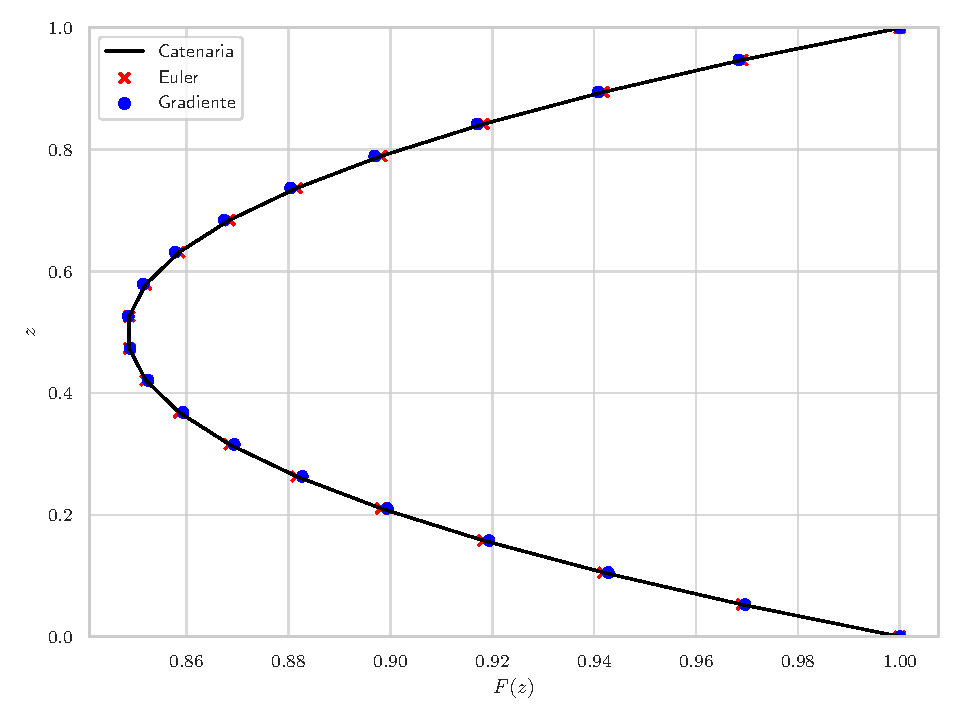
\includegraphics[width = 0.6 \linewidth]{Figuras/sol_euler.pdf}
            \end{frame}
	
	\section{Problema con restricciones de volumen}
		\begin{frame}{Problema con restricciones de volumen}
			\centering
                \begin{equation*}
                    V = \int_0^1 F^2 dz
                \end{equation*}
			\begin{minipage}[b]{0.48\textwidth}
                    \centering
                    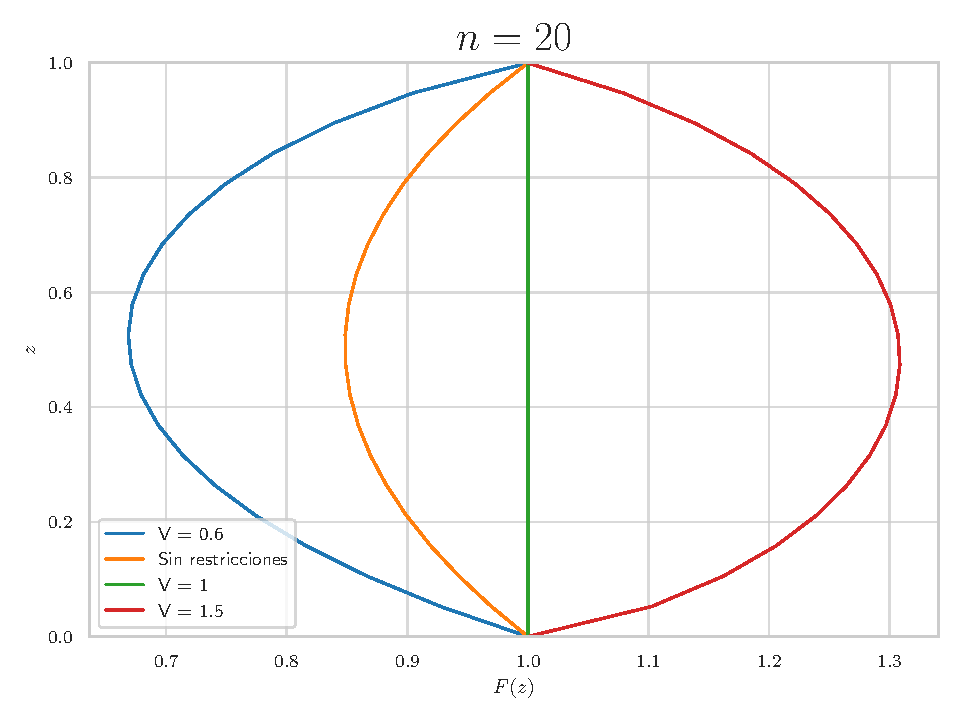
\includegraphics[height=0.5 \textheight]{Figuras/vol_inic.pdf}
                \end{minipage}
                \hfill
                \begin{minipage}[b]{0.48\textwidth}
                    \centering
                    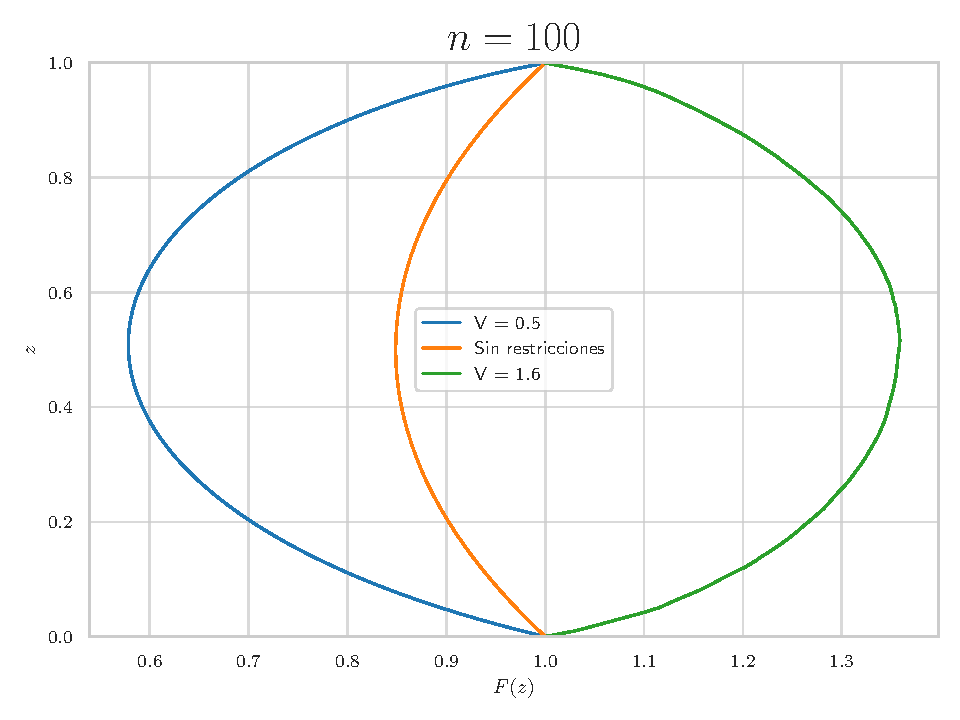
\includegraphics[height=0.5 \textheight]{Figuras/vol_sol_n100.pdf}
                \end{minipage}
		\end{frame}

            \begin{frame}{Restricciones de volumen no válidas}
                \centering
                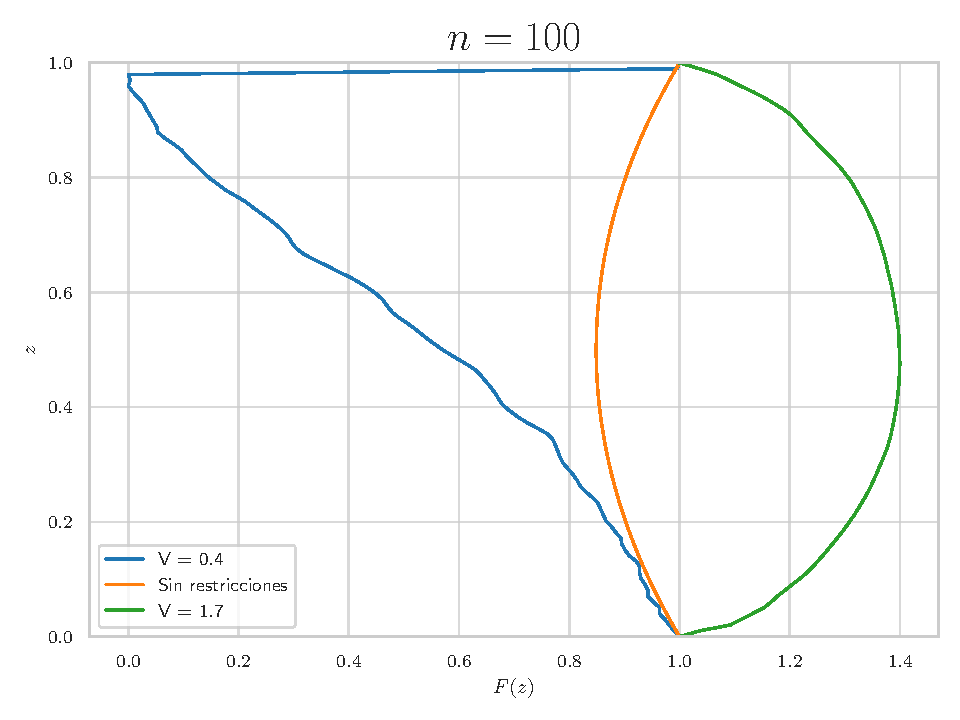
\includegraphics[width = 0.8 \linewidth]{Figuras/vol_no_sol_n100.pdf}
            \end{frame}
		
	
	\section{Problema con soportes de diferente tamaño}
		\begin{frame}{Problema con soportes de diferente tamaño}
			\centering
                \begin{equation*}
                    \begin{cases}
                        F(0) = F_0 - \varepsilon \\
                        F(1) = F_0 + \varepsilon
                    \end{cases}
                \end{equation*}
                
                \begin{minipage}[b]{0.48\textwidth}
                    \centering
                    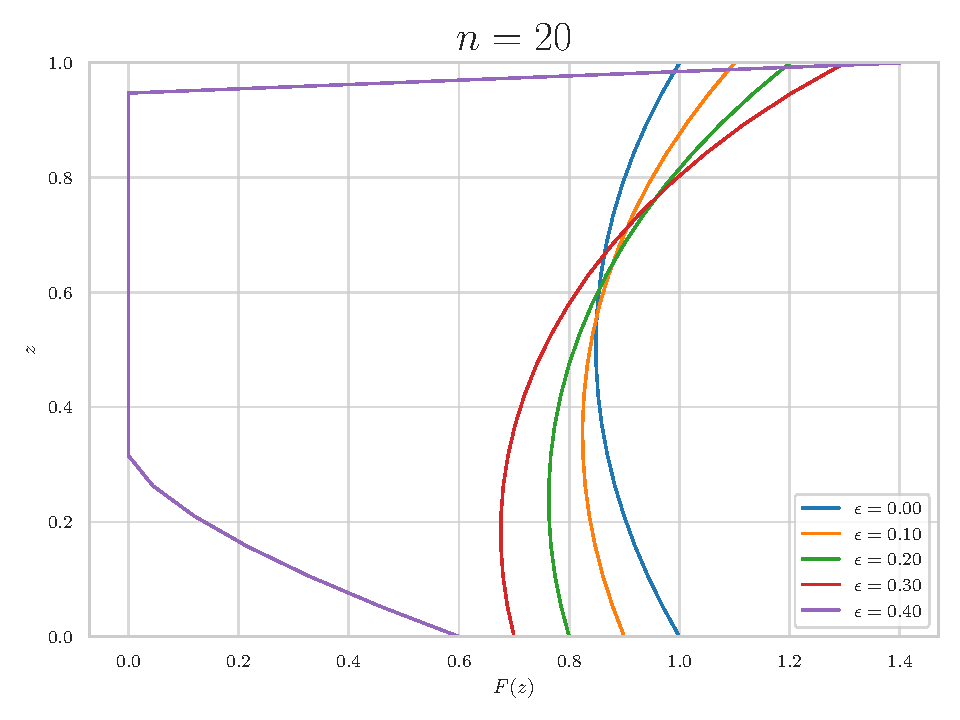
\includegraphics[height=0.5 \textheight]{Figuras/sol_var_epsn20.pdf}
                \end{minipage}
                \hfill
                \begin{minipage}[b]{0.48\textwidth}
                    \centering
                    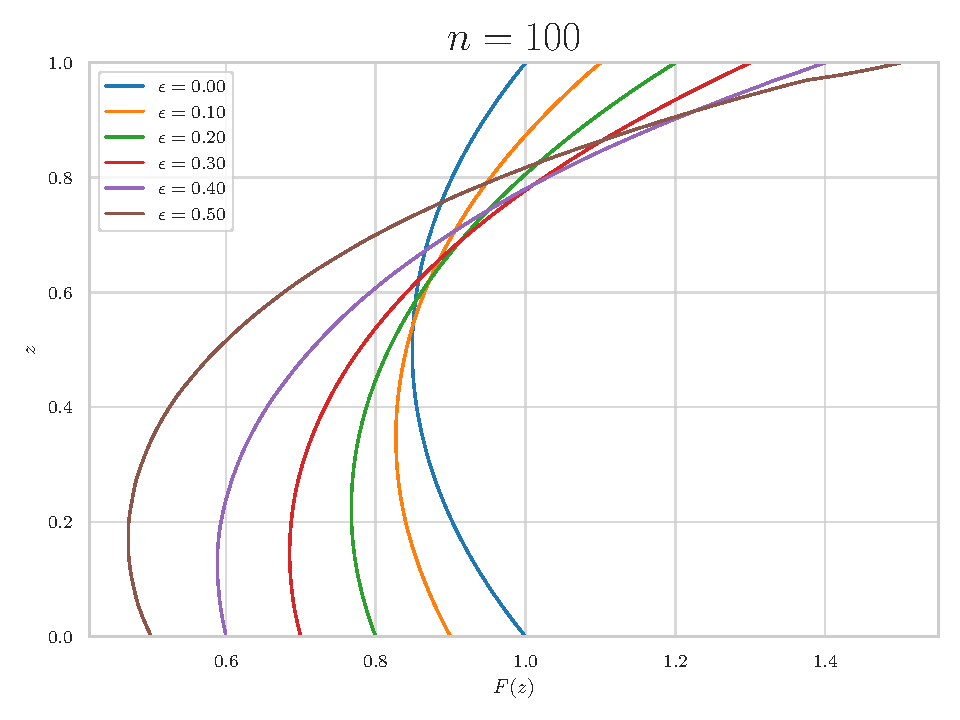
\includegraphics[height=0.5 \textheight]{Figuras/sol_var_epsn100.pdf}
                \end{minipage}
		\end{frame}

            \begin{frame}{Valores de $\varepsilon$ no válidos}
                \centering
                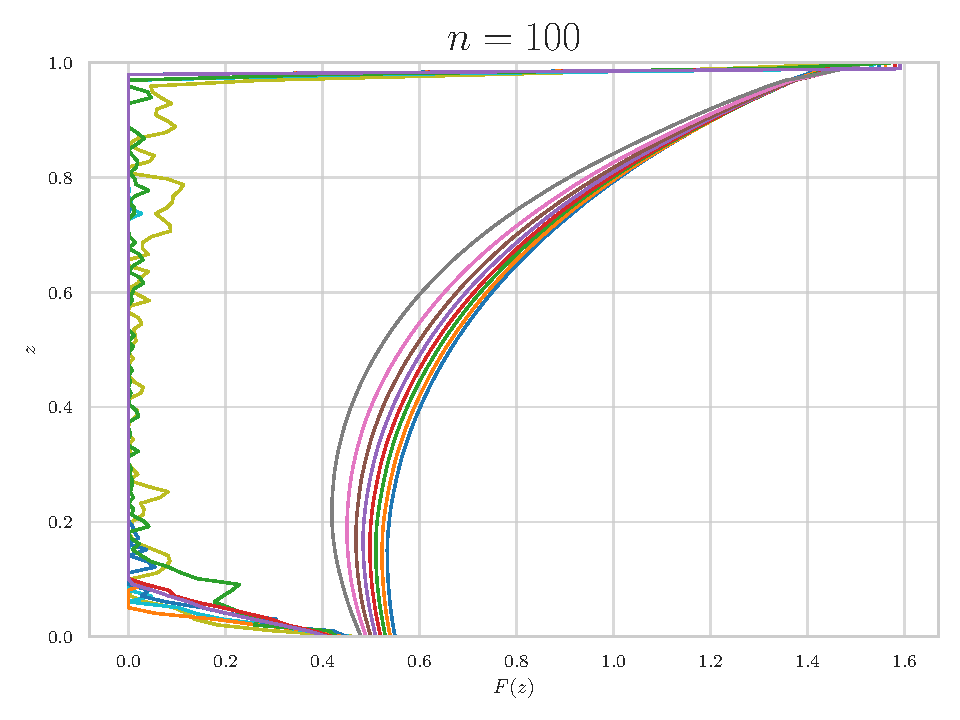
\includegraphics[width = 0.8 \linewidth]{Figuras/sol_var_epsn100_cont.pdf}
            \end{frame}

        \section{Consideraciones particulares}
            \begin{frame}{Arranque de la iteración en la solución}
            \framesubtitle{Método gradiente}
                \centering
                \begin{tabular}{|c|c|c|c|}
                    \hline
                    \textbf{Tolerancia} & \textbf{Iteraciones} & \textbf{Norma del gradiente} & \textbf{SLE [\%]} \\ \hline \hline
                    1e-05 &  1 & 6.526e-02 & 0.041 \\ \hline
                    1e-07 & 11 & 2.729e-02 & 0.085 \\ \hline
                    1e-10 & 22 & 1.453e-05 & 0.095 \\ \hline
                    1e-13 & 24 & 2.779e-06 & 0.095 \\ \hline
                    1e-16 & 69 & 7.489e-07 & 0.095 \\ \hline
                \end{tabular}                
            \end{frame}

        \section{Conclusiones}
            \begin{frame}{Conclusiones}
            \justifying
            \begin{itemize}
                \item Métodos tipo gradiente vs heurísticos
                \item Compromiso precisión vs coste computacional
                \item Influencia de los parámetros del problema
            \end{itemize}
                
            \end{frame}
	

% %\appendix
% \section{Referencias}
% %\subsection<presentation>*{Referencias}

% \begin{frame}{Referencias}

% \begin{thebibliography}{10}
	
% 	\beamertemplatearticlebibitems
% 	% imagen de libro
	
% 	\bibitem{articulo}
% 	Ginger Gardiner
% 	\newblock{\em \href{https://www.compositesworld.com/articles/in-situ-composites-sensors-for-increased-production-rates-smart-processes-and-life-cycle-monitoring}{In-situ composites sensors for increased production rates, smart processes and life cycle monitoring}}.
% 	\newblock{CompositesWorld. 23/11/2021.}
	
	
% 	% \beamertemplatebookbibitems
% 	% % imagen de revista, paper o artículo
	
% 	% \bibitem{Author19901}
% 	% Kanischka Perera.
% 	% \newblock{\em Nontrivial groups in p-Laplacian problems via the Yang index}.
% 	% \newblock{The \LaTeX\ Companion. In Topol. Methodos Nolinear Anal. 21.2 (2003) , pp 301-303}
	
	
% 	% \beamertemplateonlinebibitems
% 	% % imagen de una URL de internet
	
% 	% \bibitem{Author2019}
% 	% Aprendiendo \LaTeX
% 	% \newblock{\em Página de Facebook}.
% 	% \newblock{Manuel Merino}
	
	
	
	
	
% \end{thebibliography}
% \end{frame}
\end{document}